
\documentclass[a4paper,fleqn,usenatbib]{mnras}
\usepackage[T1]{fontenc}
\usepackage{ae,aecompl}
%%%%% AUTHORS - PLACE YOUR OWN PACKAGES HERE %%%%%
\usepackage{amstext}
\usepackage{url}
% Only include extra packages if you really need them. Common packages are:
\usepackage{graphicx}	% Including figure files
\usepackage{amsmath}	% Advanced maths commands
\usepackage{amssymb}	% Extra maths symbols
\usepackage{multirow}

%\def\elabel#1{\label{eq:#1}\fbox{#1}}
\def\elabel#1{\label{eq:#1}}

\title[Working Log: Use Deep Learning Technology to Find Strong Lensing Sources]{Use Deep Learning Technology to Find Strong Lensing Sources}
\author[He]
	{authors$^1,^2$ \thanks{E-mail: leaveformoon@hotmail.com}\\
$^1$ South-Western Institute for Astronomy Research, Yunnan University, Kunming, P.R.China\\
$^2$ Yunnan Observatory, CAS, Kunming, P.R.China
}

\date{Accepted XXX. Received YYY; in original form \today}
\pubyear{2018}


\begin{document}
\label{firstpage}
%\pagerange{\pageref{firstpage}--\pageref{lastpage}}
\maketitle

\section{Introduction}
\section{Training Samples}
\subsection{Lensing Model}
We assume the dark matter halo profile fits the Singular Isothermal Ellipsity (SIE) model.
\subsection{Positive Samples}
To train our network, we need to generate a great number of pictures that looks like actul lensed galaxies, which are called 'positive samples'. The basic idea here is that we simulated the process that the light be curved by foreground galaxies. To cover more possiblities, we change the parameters used in the program and got images of different morphologies. The overall procedure are plotted in figure1.\\
The parameters we adjusted are including:the ellipticity of dark matter halo, $e$; the ratio of the angluar distance between observer and foreground with the angluar distance between background galaxies and observer, $D_{l}/D_s$; velocity dispersion of the foreground galaxies, $\sigma_v$; the offset of the the centre of foreground and background galaxies $x,y$; the Sersic index of background galaxies, $n_s$ and the magnitude of background galaxies, $mag$.\\
\subsubsection{Ray-tracing program}
\subsubsection{Background galaxies}
We made the distribution of background galaxies conform to CANDLES COSMOS. The data we used include about 4,000 galaxies. Some features about those galaxies are plotted in figure3 and figure4. 

\subsubsection{Noises that be considered}
In our simulation, we considered following kinds of noise. At the first place, the influence of atmoshperic disturbance and instrument interference were simulated by adding Point Spread Function(PSF) to the image. To do that, we firstly choose a kernel, in this case, Airy function was used. 
\begin{center}
\begin{equation}
P(x)=\frac{I_0}{(1-\epsilon^2)^2}(\frac{2J_1(x)}{x}-\frac{2\epsilon{J_1(\epsilon{x})}}{x})^2,
\end{equation}
\end{center}
where $I_0$ is the maximum intensity at the centre, $\epsilon$ is the aperture obscuration ratio, and $J_1(x)$ is the first kind of Bessel function of order one; $x$ is defined as $x=\pi\theta/(\lambda{D})$. In our simulation, we set $D$ equal 1.2m and $\epsilon$ equal 1/3.
Then we do Fast Fourier Transform(FFT) to the original image and multiply by kernel. After that, we do inverse FFT to get image after PSF.\\
The next noise we considered is Poission noise, it is induced by the nonuniform of the distribution of photon. At program, we add a random number that fits to Poission distritbution to each pixel, with the distribution's mean equals to the intensity at certain pixel.\\
Finally, CCD read out noise and dll background were simulated by Gaussian noise. And we let the snr conform to the fit of mag-snr distribution.
\subsubsection{Foreground galaxies}
We also use Sersic profile to plot the foreground galaxies and we choose the total lumnosity equals 2 to 11 dozen times than the total lumosity of $\theta$ plane. For half light radius, we set them 0.5 to 2.5 times than $\theta_E$. For Sersic index, we choose a random number between 1 and 2.
\subsubsection{Performence}
The program needs 1.184s to generate a image under the circumstance that have CORE i5-8250U as CPU. 

\subsection{Negative Samples}
Three parts of samples have been considered. Firstly, the Gaussian white noise; secondly, the Sersic profiles that are unlensed; thirdly, real galaxies from HST. The Gaussian white noise have the ratio of 1/6, the Sersic profile have the ratio of 1/3, the real HST images have the ratio of 1/2. Since there is no lens anymore, $\sigma_v$ is needless, we then set the other parameters all same with the parameters we used for the positive samples(except for the selection of range, we set the range of image to 6(not the field, but the range of ploting image). 
The Gaussian white noise is added since we think there maybe some photos that have very low SNR so the galaxies cannot be recognized. 
For the real galaxies from HST, we add them because that we think some galaxies that have irregular shape maybe mistake for lensd galaxies. These ten galaxies are selected because their relatively abnormal shape. On the premise that integrity of shapes of galaxies is guaranteed, the images of real galaxies have been tailored randomly to increase the size of the set. Also we rotate the images by 0, 90 180, 270 dgrees randomly. After tailoring and rotating, we lower down the resolution to make sure they have the same resolution with our positvie samples.
As for unlensed Sersic galaxies, serveal galaxies were plotted instead of one. Since we want to the Network can distinguish multiply images and two normal galaxies in one image. And the number of Sersic galaxies is randomly distributed from one to three. We also sheared the image of galaxies to simulate the elliptical galaxies. 
\section{Network}
\section{Results}
For testing our network, we generate xxx png files for positive samples and xxx png files for negative samples, the total number of png files are xxx. Additionally, we equaled the size of negative samples and positive samples, by removing the extra samples randomly. For spliting training and test set, we set the ratio of test set to 1/3 and the ratio of training set to 2/3(that means the size of test set is xxx and the size of training set is xxx) and we splited the images randomly. The accuracy and ROC curve are recorded at figure6.
\section{Conclusion}

\begin{table}
	
	\centering
	
	\begin{tabular}{c|c|c|c|c|c|c|c|c|c}
		\hline
		\multicolumn{2}{|c|}{$e$} & \multicolumn{2}{|c|}{$\sigma_v(km/s)$}& \multicolumn{1}{|c|}{$n_{bias}$}
		\\
		\cline{6-10}
		lower & upper &  lower & upper\\
		\hline
		0.7 & 1.0 & 250 & 250 & 0.5 \\
		\hline
		\multicolumn{2}{|c|}{$magnitude$} & \multicolumn{2}{|c|}{$n_{sersic}$} & \multicolumn{2}{|c|}{$D_{ls}/D_s$}
		\\
		\cline{6-10}
		upper & lower & upper & lower\\
		\hline
		21 & 22.5 & 1.0 & 1.5 & 0.9\\
		\hline
	\end{tabular}
	\caption{\label{pos_set3}Parameter space for positive samples. All the parameters are select uniformly, with the step of ellipticity equals to 0.1, step of $magnitude$ equals to 0.1, step of $n_{bsersic}$ equals to 0.1. The step of coordinates of bias of localtion is 0.1 $arcsec$.}
\end{table}

\begin{figure}
\centerline{
  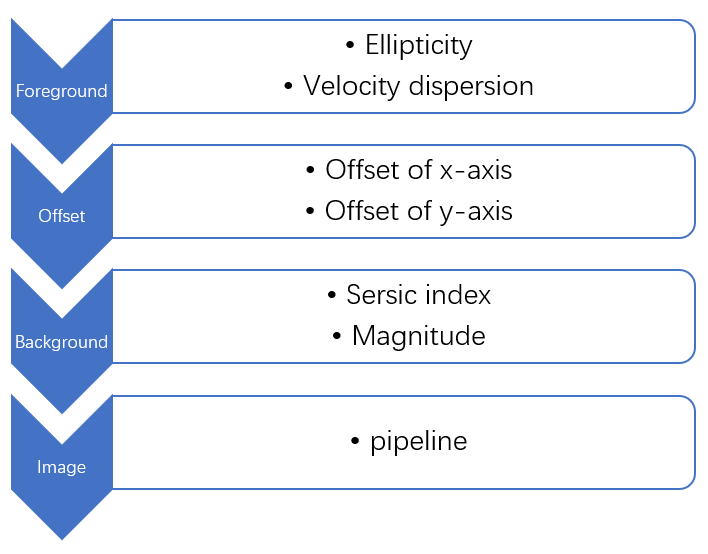
\includegraphics[scale=0.3]{procedure.png}}
  \caption{Overall procedure}
\label{figProcedure}
\end{figure}

\begin{figure}
\centerline{
  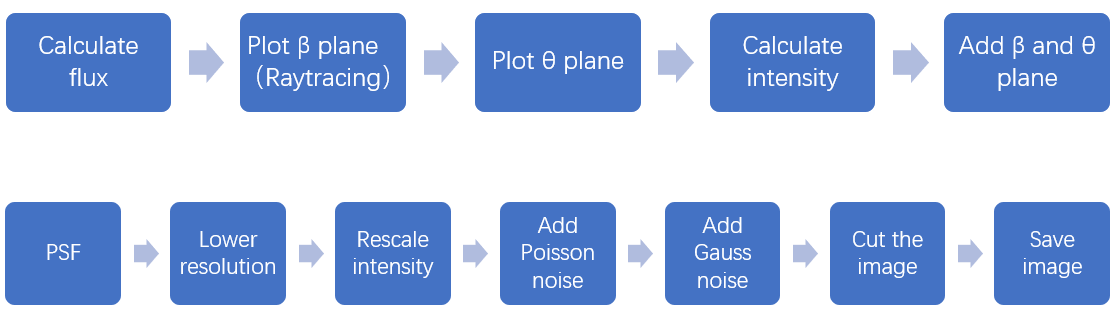
\includegraphics[scale=0.3]{pipeline.png}}
  \caption{Pipeline of generating a image.}
\label{figPipeline}
\end{figure}

\begin{figure}
  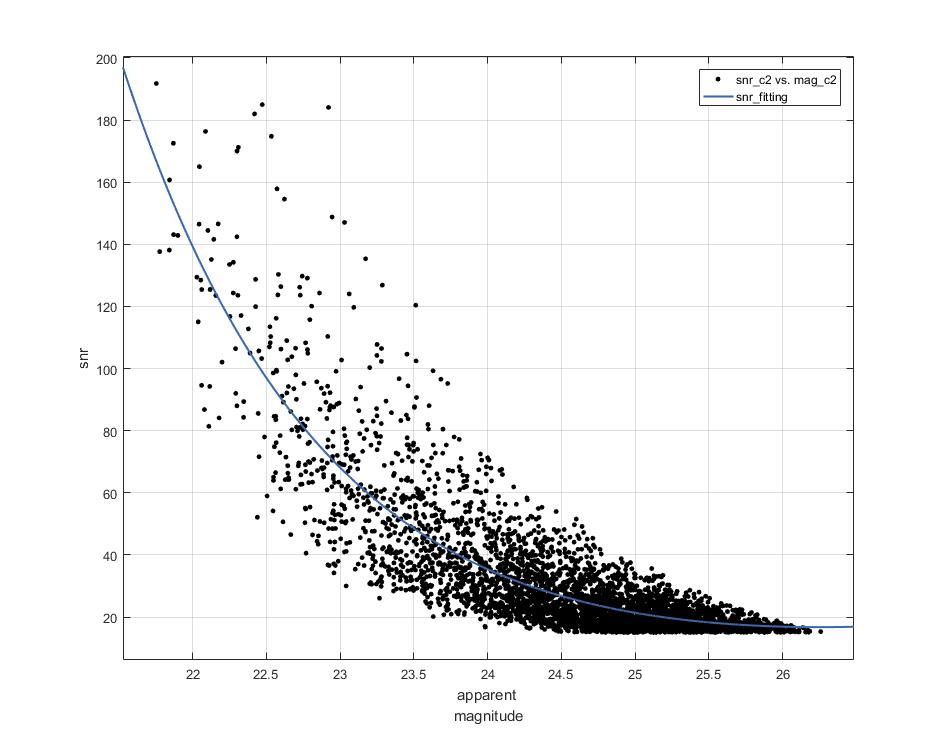
\includegraphics[scale=0.12]{fitting_of_snr.jpg}
  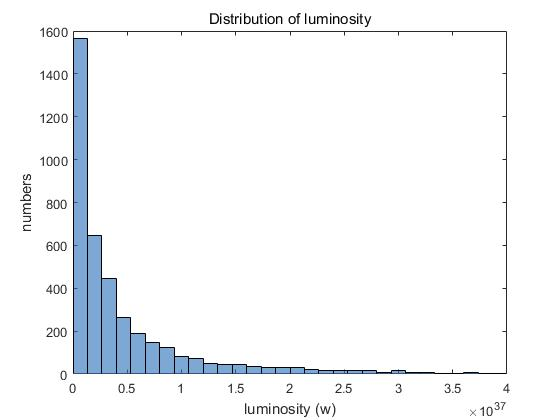
\includegraphics[scale=0.23]{distribution_of_lum.jpg}
  \caption{Features of data.}
\label{figMagDistribution}
\end{figure}

\begin{figure}
  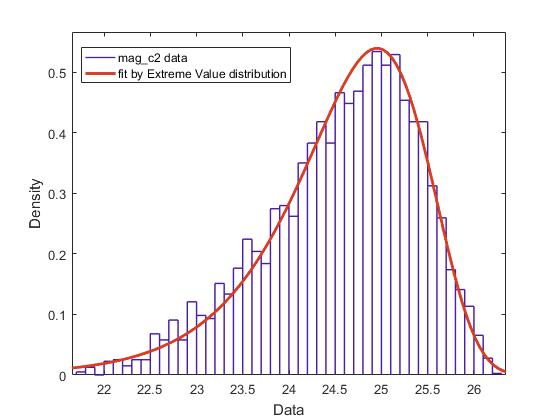
\includegraphics[scale=0.21]{fig_of_mag.jpg}
  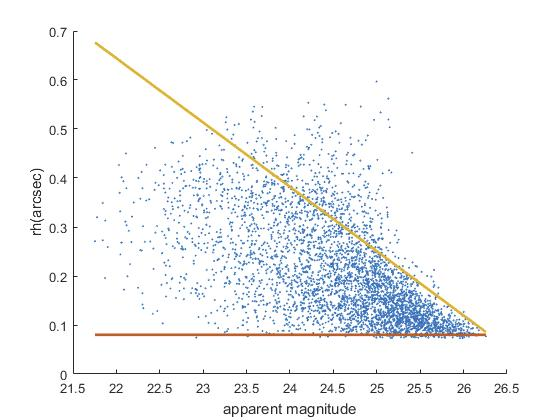
\includegraphics[scale=0.21]{fitting_of_rh.jpg}
  \caption{Fitting of data.}
\label{figMagDistribution}
\end{figure}

\begin{figure}

  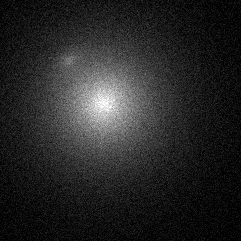
\includegraphics[scale=0.4]{ps1.png}
  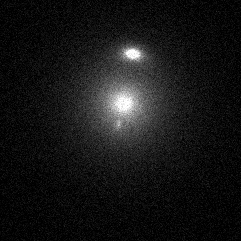
\includegraphics[scale=0.4]{ps2.png}
  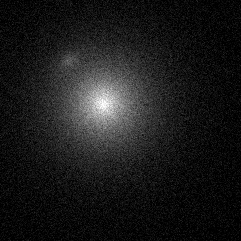
\includegraphics[scale=0.4]{ps3.png}  
  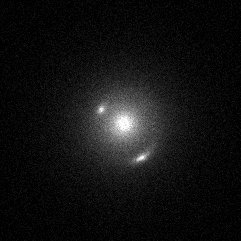
\includegraphics[scale=0.4]{ps4.png}
  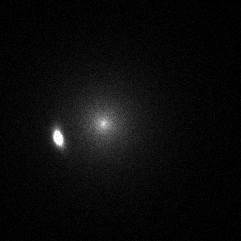
\includegraphics[scale=0.4]{p5.png}
  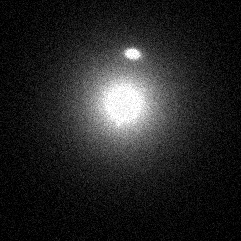
\includegraphics[scale=0.4]{p6.png}
  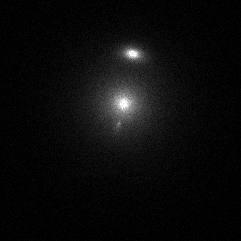
\includegraphics[scale=0.4]{p7.png}
  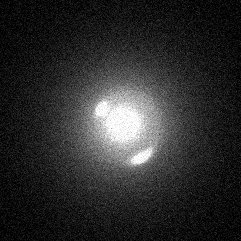
\includegraphics[scale=0.4]{p8.png}
  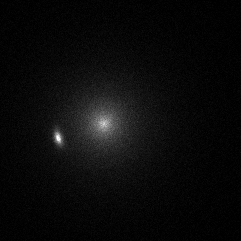
\includegraphics[scale=0.4]{p9.png}
  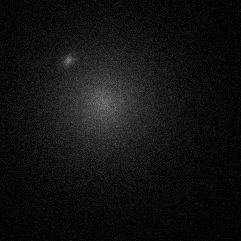
\includegraphics[scale=0.4]{p10.png}
  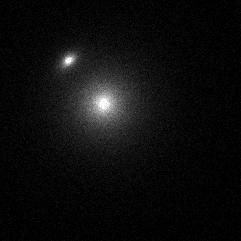
\includegraphics[scale=0.4]{p11.png}
  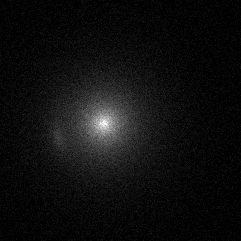
\includegraphics[scale=0.4]{p12.png}

  \caption{Some exmpales of positive samples.}
\label{ps}
\end{figure}
\end{document}





















